% !TEX root = ../YourName-Dissertation.tex

\chapter{Development of Resonant Cavities for Large Volume CRES Measurements}

\section{Introduction}

The cavity approach is an alternative CRES measurement technology under consideration by the Project 8 collaboration for a neutrino mass measurement experiment with 40~meV sensitivity. After pursuing an antenna array based CRES demonstrator design for several years the increasing costs and complexity of the antenna arrays led to a rexamination of resonant cavities for a large scale experiment. Currently, a cavity based CRES experiment is the preferred technology for the Project 8 neutrino mass measurement goal with antennas as a fall-back approach. 

In this chapter we provide a brief summary of resonant cavities and sketch out the key features of a cavity based CRES experiment. In Section \ref{sec:chap6-resonant-cavities} we provide a brief introduction to cylindrical resonant cavities and the solutions for the electromagnetic fields in the cavity volume.

In Section \ref{sec:chap6-cavity-approach} we describe the main components of a cavity based CRES experiment. Including the background and trap magnets, cavity geometry and design, and cavity coupling considerations. We also discuss some relevant trade-offs between an antenna array and cavity CRES experiment, and highlight some reasons for the transition of Project 8 to the development of a cavity based experiment.

Finally, in Sections \ref{sec:chap6-single-mode-cavity-sims} and \ref{sec:chap6-single-mode-cavity-measurement} I present the design and development of an open, mode-filtered cavity that could be used in a cavity based CRES experiment. The results of the cavity simulations are confirmed by laboratory measurements of a proof-of-principle prototype cavity intended to demonstrate key features of the design.

\section{Cylindrical Resonant Cavities}
\label{sec:chap6-resonant-cavities}

Resonant cavities are essentially sealed conductive containers, which allows us to describe the electromagnetic (EM) fields as a superposition of resonant modes. The field shapes of the resonant modes are determined by Maxwell's equations and the boundary conditions enforced by the cavity geometry. Of interest to Project 8 for CRES measurements are cylindrical cavities due to their ease of construction and integration with atom and electron trapping magnets. 

\subsection{General Field Solutions}

Consider a long segment of conducting material with a cylindrical cross-section (see Figure \ref{fig:chap6-circ-waveguide}). A geometry such as this can be used as a waveguide transmission line to transfer EM energy from point to point, or, if conducting shorts are inserted on both ends of the cylinder, the waveguide becomes a resonant cavity. 

\begin{figure}[htbp]
    \centering
    \includegraphics*[width=0.4\textwidth]{figs/Chapter-6/230606_circular_waveguide.png}
    \caption{\label{fig:chap6-circ-waveguide} Geometry of a cylindrical waveguide with radius $b$. }
\end{figure}

The fields allowed inside a cylindrical cavity are determined by the boundary conditions of the cylindrical geometry. The general approach to solving for the fields begins by assuming solutions to Maxwell's equations of the form
\begin{align}
    \label{eq:chap6-maxwell-eqn-solutions-E}\bm{E}(x,y,z)&=(\bm{e}(x,y)+\hat{z}e_z(x,y))e^{-i\beta z},\\
    \label{eq:chap6-maxwell-eqn-solutions-H}\bm{H}(x,y,z)&=(\bm{h}(x,y)+\hat{z}h_z(x,y))e^{-i\beta z}.
\end{align}

The solutions assume a harmonic time dependence of the form $e^{i\omega t}$ and propagation along the positive z-axis. The functions $\bm{e}(x,y)$ and $\bm{h}(x,y)$ represent the transverse ($\hat{x}, \hat{y}$) components of the electric and magnetic fields respectively, and $e_z(x,y)$, $h_z(x,y)$ are the longitudinal components. The version of Maxwell's equations in the case where there are no source terms can be written as a pair of coupled differential equations, 
\begin{align}
    \nabla\times\bm{E}&=-i\omega\mu\bm{H},\\
    \nabla\times\bm{H}&=i\omega\epsilon\bm{E},
\end{align}
where $\epsilon$ and $\mu$ are the permittivity and permeability of the material inside the waveguide or cavity. Using the field solutions from Equations \ref{eq:chap6-maxwell-eqn-solutions-E} and \ref{eq:chap6-maxwell-eqn-solutions-H} one can solve for the transverse components of the fields in terms of the longitudinal fields. Because we are interested in cylindrical cavities it is advantageous to write the field solutions in cylindrical coordinates. After performing this transformation the set of four equations for the transverse field components are,
\begin{align}
    H_\rho&=\frac{i}{k_c^2}\left(\frac{\omega\epsilon}{\rho}\frac{\partial E_z}{\partial \phi}-\beta \frac{\partial H_z}{\partial \rho}\right),\\
    H_\phi&=\frac{-i}{k_c^2}\left(\omega\epsilon\frac{\partial E_z}{\partial \rho}+\frac{\beta}{\rho}\frac{\partial H_z}{\partial \phi}\right),\\
    E_\rho&=\frac{-i}{k_c^2}\left(\beta\frac{\partial E_z}{\partial \rho}+\frac{\omega\mu}{\rho}\frac{\partial H_z}{\partial \phi}\right),\\
    E_\phi&=\frac{i}{k_c^2}\left(\frac{-\beta}{\rho}\frac{\partial E_z}{\partial \phi}+\omega\mu\frac{\partial H_z}{\partial \rho}\right),
\end{align}
where $k_c$ is the cutoff wavenumber defined by $k_c^2=k^2-\beta^2$ with $k=\omega\sqrt{\mu\epsilon}$ being the wavenumber of the EM radiation. 

This set of equations can be used to solve for a variety of different modes that can be obtained by setting conditions on $E_z$ and $H_z$. For cylindrical cavities two types of modes are allowed, which correspond to solutions where $E_z=0$ and $H_z=0$ respectively. 

\subsection{TE and TM Modes}
\label{sec:chap6-TE-TM-modes}

The TE family of modes corresponds to the case where $E_z=0$. This implies that $H_z$ is a solution to the Helmholtz wave equation 
\begin{equation}
    (\nabla^2 + k^2)H_z = 0.
    \label{eq:chap6-helmholtz-magnetic}
\end{equation}
For solutions of the form $H_z(\rho,\phi,z)=h_z(\rho,\phi)e^{-i\beta z}$, Equation \ref{eq:chap6-helmholtz-magnetic} can be solved using the standard technique of separation of variables. Rather than reproduce the derivation here we shall simply quote the solutions for the transverse fields, which are 
\begin{align}
    H_\rho &= \frac{-i\beta }{k_{c_{nm}}}(A\sin{n\phi}+B\cos{n\phi})J_n^\prime(k_{c_{nm}}\rho)e^{-i\beta_{nm} z},\\
    H_\phi &=\frac{-i\beta n}{k_{c_{nm}}^2\rho}(A\cos{n\phi}-B\sin{n\phi})J_n(k_{c_{nm}}\rho)e^{-i\beta_{nm} z},\\
    E_\rho &=\frac{-i\omega\mu n}{k_{c_{nm}}^2 \rho}(A\cos{n\phi}-B\sin{n\phi})J_n(k_{c_{nm}}\rho)e^{-i\beta_{nm} z},\label{eq:chap6-erho-TE}\\
    E_\phi &=\frac{i\omega\mu}{k_{c_{nm}}}(A\sin{n\phi}+B\cos{n\phi})J_n^\prime(k_{c_{nm}}\rho)e^{-i\beta_{nm} z}\label{eq:chap6-ephi-TE}.
\end{align}
One can observe that the solutions have a periodic dependence on $\phi$, and radial profiles given by the Bessel functions of the first kind. The integer indices $n$ and $m$ arise from continuity conditions on the EM fields in the azimuthal and radial directions. For the TE modes $n\geq0$ and $m\geq1$. $k_{c_{nm}}$ is the cutoff wavenumber for the $\mathrm{TE}_{nm}$ mode given by 
\begin{equation}
    k_{c_{nm}} = \frac{p^\prime_{nm}}{b},
\end{equation}
where $b$ is the radius of the cavity or waveguide and $p^\prime_{nm}$ is the $m$-th root of the derivative of the $n$-th order Bessel function (see Table \ref{tab:chap6-bessel-derivative-roots}).

\begin{table}[htbp]
    \centering
    \caption{\label{tab:chap6-bessel-derivative-roots} A table of the values of $p_{nm}^\prime$.}
    \begin{tabular}{c c c c }
        \hline
        $n$ & $p_{n1}^\prime$ & $p_{n2}^\prime$ & $p_{n3}^\prime$ \\
        \hline
        0 & 3.832 & 7.016 & 10.174\\
        1 & 1.841 & 5.331 & 8.536\\
        2 & 3.054 & 6.706 & 9.970\\
        \hline
    \end{tabular}
\end{table}

The TM mode family corresponds to the case where $H_z=0$, and $(\nabla^2 +k^2)E_z=0$. Again, we assume solutions of the form $E_z(\rho,\phi,z)=e_z(\rho,\phi)e^{-i\beta z}$, for which the general form of the solutions is the same as for the TE modes. However, the different boundary conditions for the TM modes results in particular solutions with a different from, which we shall quote here without derivation. The transverse fields of the TM modes are given by 
\begin{align}
    H_\rho &=\frac{-i\omega\epsilon n}{k_{c_{nm}}^2 \rho}(A\cos{n\phi}-B\sin{n\phi})J_n(k_{c_{nm}}\rho)e^{-i\beta_{nm} z},\\
    H_\phi &=\frac{-i\omega\epsilon}{k_{c_{nm}}}(A\sin{n\phi}+B\cos{n\phi})J_n^\prime(k_{c_{nm}}\rho)e^{-i\beta_{nm} z}\\
    E_\rho &= \frac{-i\beta }{k_{c_{nm}}}(A\sin{n\phi}+B\cos{n\phi})J_n^\prime(k_{c_{nm}}\rho)e^{-i\beta_{nm} z},\\
    E_\phi &=\frac{-i\beta n}{k_{c_{nm}}^2\rho}(A\cos{n\phi}-B\sin{n\phi})J_n(k_{c_{nm}}\rho)e^{-i\beta_{nm} z},
\end{align}
which one may notice are the same solutions as the TE modes with $H$ and $E$ flipped. The cutoff wavenumber for the TM modes is given by, $k_{c_{nm}}=p_{nm}/b$, where the values of $p_{nm}$ correspond to the $m$-th zero of the $n$-th order Bessel function (see Table \ref{tab:chap6-bessel-roots}).

\begin{table}[htbp]
    \centering
    \caption{\label{tab:chap6-bessel-roots} A table of the values of $p_{nm}$.}
    \begin{tabular}{c c c c }
        \hline
        $n$ & $p_{n1}$ & $p_{n2}$ & $p_{n3}$ \\
        \hline
        0 & 2.405 & 5.520 & 8.654\\
        1 & 3.832 & 7.016 & 10.174\\
        2 & 5.135 & 8.417 & 11.620\\
        \hline
    \end{tabular}
\end{table}

\subsection{Resonant Frequencies of a Cylindrical Cavity}

A cylindrical cavity is essentially constructed by taking a section of cylindrical waveguide and shorting both ends with conductive material. This means that the electric fields inside a cylindrical cavity are exactly those we derived in Section \ref{sec:chap6-TE-TM-modes} with the additional condition that the electric fields must go to zero at $z=0$ and $z=L$ (see Figure \ref{fig:chap6-cyl-cav}).
\begin{figure}[htbp]
    \centering
    \includegraphics*[width=0.3\textwidth]{figs/Chapter-6/230606_cylindrical_cavity.png}
    \caption{\label{fig:chap6-cyl-cav} The geometry of a cylindrical cavity with length $L$ and radius $b$.}
\end{figure}

The transverse electric field solutions for a cylindrical waveguide are of the form
\begin{equation}
    \bm{E}(\rho,\phi,z)=\bm{e}(\rho,\phi)\left(A_+e^{-i\beta_{nm}z}+A_-e^{i\beta_{nm}z }\right),
\end{equation}
where $A_+$ and $A_-$ are arbitrary amplitudes of forward and backward propagating waves. In order to enforce that $\bm{E}$ is zero at both ends of the cavity we require that 
\begin{equation}
    \beta_{nm}L = 2\pi \ell,
\end{equation}
where $\ell=0,1,2,3\ldots$. Using this constraint on the propagation constant we can solve for the resonant frequencies of the $\mathrm{TE}_{nm\ell}$ and the $\mathrm{TM}_{nm\ell}$ modes in a cylindrical cavity. For the TE modes the resonant frequencies are
\begin{equation}
    f_{nm\ell}=\frac{c}{2\pi\sqrt{\mu_r\epsilon_r}}\sqrt{\left(\frac{p_{nm}^\prime}{b}\right)^2+\left(\frac{\ell\pi}{L}\right)^2},
\end{equation}
and the frequencies of the TM modes are 
\begin{equation}
    f_{nm\ell}=\frac{c}{2\pi\sqrt{\mu_r\epsilon_r}}\sqrt{\left(\frac{p_{nm}}{b}\right)^2+\left(\frac{\ell\pi}{L}\right)^2}.
\end{equation}

\begin{figure}[htbp]
    \centering
    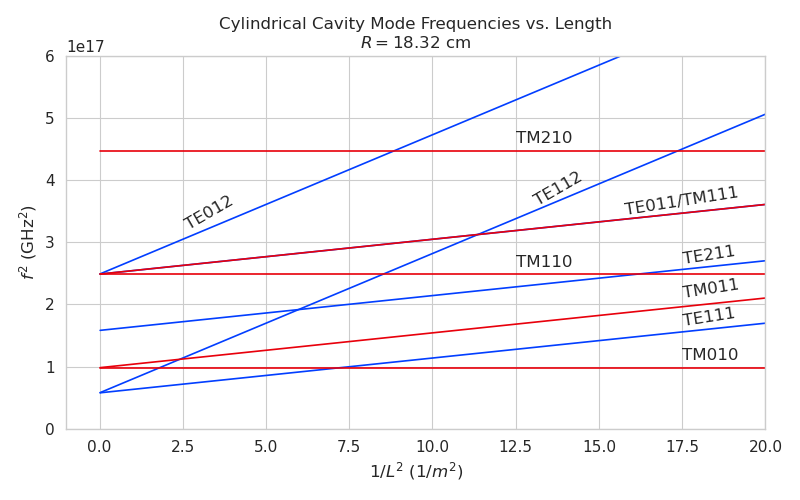
\includegraphics[width=0.75\textwidth]{figs/Chapter-6/230610_mode_lines.png}
    \caption{\label{fig:chap6-cavity-mode-lines} Relation of mode frequency to cavity length for a cylindrical cavity with a radius of 18.32~cm.}
\end{figure}

\subsection{Cavity Q-factors}

\begin{figure}[htbp]
    \centering
    \includegraphics*[width=0.6\textwidth]{figs/Chapter-6/230607_rlc.png}
    \caption{\label{fig:chap6-series-rlc} A series RLC circuit.}
\end{figure}

The resonant behavior of cylindrical cavities can be modeled as a series RLC circuit (see figure \ref{fig:chap6-series-rlc}). The input impedance of the circuit can be obtained by applying Kirchhoff's laws to calculate the impedance of the equivalent circuit. For a series RLC circuit the input impedance is 
\begin{equation}
    Z_\mathrm{in}=\left(\frac{1}{R}+\frac{1}{i\omega L}+i\omega C\right).
\end{equation}
The resistance in the circuit represents all sources of loss in the cavity, which is primarily caused by the finite conductivity of the cavity walls, and the inductor and capacitor represent the energy stored in the cavity in the form of electric and magnetic fields. If the circuit is being driven by an external power source we can write the input power in terms of the circuit input impedance and the source voltage 
\begin{equation}
    P_\mathrm{in} = \frac{1}{2}Z_\mathrm{in}|I|^2=\frac{1}{2}|I|^2\left(\frac{1}{R}+\frac{1}{i\omega L}+i\omega C\right).
\end{equation} 
The resistor introduces a loss into the system with a power given by 
\begin{equation}
    P_\mathrm{loss} = \frac{1}{2}|I|^2R,
\end{equation}
and the capacitor and inductor store energies given by
\begin{align}
    W_e&=\frac{1}{4}\frac{|I|^2}{\omega^2 C},\\
    W_m&=\frac{1}{4}|I|^2 L,
\end{align}
respectively. Using these expressions we can write the input power and input impedance expressions in terms of the lost power and stored energy 
\begin{align}
    P_\mathrm{in}=P_\mathrm{loss}+2i\omega(W_m-W_e),\\
    Z_\mathrm{in}=\frac{P_\mathrm{loss}+2i\omega(W_m-W_e)}{\frac{1}{2}|I|^2}.
\end{align}

The condition for resonance in the RLC circuit is that the stored magnetic energy is equal to the stored electric energy ($W_e$=$W_m$). When this occurs $Z_\mathrm{in}=R$, which is a purely real impedance, and $P_{in}=P_{loss}$. The resonant frequency of the circuit can be determined from the condition $W_e=W_m$ from which one finds that 
\begin{equation}
    \omega_0=\frac{1}{\sqrt{LC}}.
\end{equation}
An important performance parameter for any resonant system is the Q-factor, which quantifies the quality of the resonator as the ratio of the stored energy multiplied by the resonant frequency to the average energy lost per second. For the series RLC circuit, the Q-factor is given by the expression 
\begin{equation}
    Q_0=\omega\frac{W_e+W_m}{P_\mathrm{loss}}=\frac{1}{\omega_0RC},
\end{equation}
from which one observes that as the resistance of the RLC circuit is decreased the quality factor of the resonator increases. From the perspective of cylindrical cavities this implies that as one decreases the resistance of the cavity walls it is expected that the Q-factor of the cavity should increase, which is indeed the case. In certain applications where a high Q is desireable it is possible to manufacture a cavity out of superconducting materials in order to minimize the power losses of the system.

\begin{figure}[htbp]
    \centering
    \includegraphics*[width=0.6\textwidth]{figs/Chapter-6/230607_rlc_resonance.png}
    \caption{\label{fig:chap6-rlc-resonance} Illustration of the behavior of the input impedance of the series RLC circuit as a function of the driving frequency. The BW is proportion to the width of the resonance, which is inversely proportional to Q.}
\end{figure}

The Q-factor of the resonator also determines with bandwidth (BW) of the system. A cavity with a high Q-factor will resonant with a smaller range of frequencies than a cavity with a low Q-factor. To see this we can examine the behavior of the RLC circuit when driven by frequencies near the resonance. For a frequency $\omega=\omega_0+\Delta \omega$, where $\Delta \omega=\omega-\omega_0\ll \omega_0$, we can write the input impedance as 
\begin{equation}
    Z_\mathrm{in}=R+i\omega L\left(\frac{\omega^2-\omega_0^2}{\omega^2}\right),
\end{equation}
and by expanding $(\omega^2-\omega_0^2)/\omega^2$ to first order in $\Delta\omega$, we obtain 
\begin{equation}
    Z_\mathrm{in}\approx R+i\frac{2RQ_0\Delta\omega}{\omega_0}.
\end{equation}
Therefore, the magnitude of the input impedance near the resonance is given by 
\begin{equation}
    |Z_\mathrm{in}|=R\sqrt{1+4Q_0^2\frac{\Delta\omega^2}{\omega^2}}, 
    \label{eq:chap6-mag-input-impedance}
\end{equation}
from which we observe that for the series RLC circuit the input impedance is minimized at the resonant frequency, which corresponds to the maximum input power (see Figure \ref{fig:chap6-rlc-input-impedance}). The half-power BW is the range of frequencies over which the input power drops to half the input power on resonance. This occurs when $|Z_\mathrm{in}|=\sqrt{2}R$, which corresponds to $\Delta\omega/\omega=\textrm{BW}/2$. Using Equation \ref{eq:chap6-mag-input-impedance} one can find that
\begin{equation}
    2R^2=R^2(1+Q_0^2\mathrm{BW}^2),
\end{equation}
which implies
\begin{equation}
    \mathrm{BW}=\frac{1}{Q_0}
\end{equation}

\begin{figure}[htbp]
    \centering
    \includegraphics*[width=0.7\textwidth]{figs/Chapter-6/230607_loaded_rlc.png}
    \caption{\label{fig:chap6-loaded-resonator-circuit} A series RLC circuit coupled to an external circuit with input impedance $R_L$.}
\end{figure}

It is important to emphasize that the Q-factor defined here, $Q_0$, is technically the unloaded Q. It reflects the quality of the cavity or resonant circuit without the influence of any external circuitry. In practice, however, a cavity is invariably coupled to an external circuit to drive a cavity resonance or to measure the energy of a resonant mode. Coupling a cavity to an external circuit changes the Q by loading the equivalent cavity RLC circuit (see Figure \ref{fig:chap6-loaded-resonator-circuit}). The Q-factor of the cavity when it is loaded by an external circuit is called the loaded Q, which is the quantity that one actually measures when exciting a resonance in the cavity. Using the series RLC circuit model one can see that the load resistor in Figure \ref{fig:chap6-loaded-resonator-circuit} will add in series with the resistor in the circuit for a total equivalent resistance of $R+R_L$. Therefore, the loaded Q is given by 
\begin{equation}
    Q_L=\frac{1}{\omega_0(R+R_L)C},
\end{equation}
from which one observes that the loaded Q is always less than the intrinsic Q of the cavity.

The amount of coupling that is desireable depends on the specific application of the resonator. If one wants a resonator that is particular frequency selective than it makes sense to limit the amount of coupling to the cavity to maintain a small BW, alternatively, if a larger BW is need one can increase the cavity coupling by tuning the input impedance of the external circuit. The critical point, where maximum power is transferred between the cavity and the external circuit, occurs when the input impedance of the cavity matches the input impedance of the external transmission line.  For the series RLC circuit on resonance, this matching condition corresponds to 
\begin{equation}
    Z_0=Z_\mathrm{in}=R,
\end{equation}
where $Z_0$ is the impedance of the transmission line. The loaded Q at this critical point is, therefore,
\begin{equation}
    Q_L=\frac{1}{2\omega_0Z_0C}=\frac{Q_0}{2}.
\end{equation}
One can described the degree of coupling between the cavity and an external circuit by defining a coupling factor, $g$, such that,
\begin{equation}
    g=\frac{Q_0}{Q_L}-1.
\end{equation} 
When $g=1$ then $Q_L=Q_0/2$, and the cavity is said to be critically coupled as we described. If $Q_L<Q_0/2$, then the cavity is undercoupled to the transmission line, corresponding to $g<1$. Alternatively, if $Q_L>Q_0/2$, then $g>1$, and the cavity is overcoupled to the transmission line. Various specialized circuits can be used to tune the input impedance of the external circuit as seen by the cavity to achieve a wide range of different coupling factors based on the desired application of the cavity.

\section{The Cavity Approach to CRES}
\label{sec:chap6-cavity-approach}

\subsection{A Sketch of a Molecular Tritium Cavity CRES Experiment}

Resonant cavities can be used to perform CRES measurements, and they represent the current preferred technology by the Project 8 collaboration for the ultimate goal of a 40~meV neutrino mass measurement using CRES. The basic approach to a neutrino mass measurement using a resonant cavity and molecular tritium beta-decay source is illustrated by Figure \ref{fig:chap6-cav-cartoon}.
\begin{figure}[htbp]
    \centering
    \includegraphics*[width=0.7\textwidth]{figs/Chapter-6/230606_cavity_cartoon.png}
    \caption{\label{fig:chap6-cav-cartoon} Cartoon depiction of a cavity CRES experiment.}
\end{figure}

At the core of the experiment is a large resonant cavity filled with tritium gas. In principle a sealed metallic cavity serves a dual purpose as the tritium containment vessel although the risks of exposure to radioactive tritium may necessitate a secondary dielectric containment vessel (such as fused scilica) inside the cavity volume. The filled cavity is then placed in a uniform magnetic field provided by a primary magnet that sets the values of the cyclotron frequencies for electrons emitted with energies near the tritium spectrum endpoint. When a beta-decay electron is produced in the cavity it is trapped using an additional set of magnetic coils that prevents the electrons from running into the cavity walls.

Electrons trapped inside the cavity volume do not radiate in the same way as electron in free-space. Effectively, the same boundary conditions that were used to derive the resonant modes of a cylindrical cavity in Section \ref{sec:chap6-resonant-cavities} apply to the radiation of the electron as well. If an electron is emitted with a kinetic energy that corresponds to a cyclotron frequency that matches a resonant frequency of the cavity, then the power radiated by the electron excites the corresponding resonance in the cavity. The strength of the electron's coupling to the cavity is given by the dot product between the electrons trajectory and the electric field vector of the resonant mode. However, if an electron is moving with a cyclotron frequency that is far from any resonant modes in the cavity, then radiation from the electron is suppressed. One can interpret this somewhat surprising effect as the metallic walls of the cavity reflecting the radiated energy back into the electron. 

To detect the electron the cavity is coupled to an external transmission line that leads to an amplifier and RF receiver chain similar to an antenna array based experiment. The coupling of the cavity resonance to the amplifier occurs through a coupling probe designed to resonate with the same mode or modes excited by the electron. In other resonant cavity systems this is often accomplished using a simple wire antenna,  which could be connected to the amplifier through a segment of coaxial cable. Alternatively, cavities are oftentimes coupled to waveguides or smaller external cavities using small holes or apertures cut into the main cavity wall. For CRES measurements, the placement of a wire coupling probe inside the cavity volume leads to additional scattering of electrons and eventually tritium atoms, therefore, the apertures are the preferred coupling method for cavity CRES experiments.

One of the attractive features of the CRES technique for neutrino mass measurement is the gain in statistics that comes from the differential nature of the tritium spectrum measurement. Initially, this seems incompatible with cavities, due to the narrow resonances of cavity modes giving relatively small bandwidth. However, by intentionally overcoupling to a single cavity mode one can achieve bandwidths of a few 10's of MHz, which is sufficient for a measurement of the tritium spectrum endpoint region.  

\subsection{Magnetic Field, Cavity Geometry, and Resonant Modes}

\subsubsection*{Magnetic Field and Volume Scaling}

For a CRES experiment, cylindrical cavities are a natural choice since they match the geometry of standard solenoid magnets, which are needed in order to produce the background magnetic field for CRES measurements. Furthermore, the cylindrical shape is compatible with a Halbach array, which is the leading choice of atom trapping technology for future atomic tritium experiments by the Project 8 collaboration. Cylindrical cavities also benefit from well-established machining practices that are able to achieve high geometric precision at large lengths scales. Currently, a cylindrical cavity is the preferred cavity shape for CRES measurements by Project 8, although, there are on-going efforts to investigate more complicated cavity designs that may offer advantages over the more standard geometry.

As we saw in Section \ref{sec:chap6-resonant-cavities}, the physical dimensions of the cavity are directly coupled to the resonant frequencies of the cavity. This dependency links the size of the cavity to the magnitude of the background magnetic field, because the magnetic field determines the cyclotron frequencies of trapped electrons. Specifically, as the size of the cavity is increased to accommodate larger volumes of tritium gas, the wavelengths and frequencies of the resonant modes increase and decrease respectively. This requires that the magnetic field also decrease in order to maintain coupling between electrons and the desired cavity mode. 

The required cavity size is ultimately determined by the required statistics in the tritium spectrum endpoint region. Because the gas density must be kept below a certain level to ensure that electrons have sufficient time to radiate before scattering, larger volumes become the only way to achieve higher event statistics. To achieve the sensitivity goals of Phase III and IV cavity volumes on the order of several cubic-meters are required, which pushes one towards frequencies in the range of 100's of MHz.

\subsubsection*{Single-mode Cavity CRES}

It is tempting to consider maintaining a high magnetic field while increasing the size of the cavity in order to increase the radiated power from trapped electrons for a potentially better SNR. However, if one were to maintain the same magnetic field while increasing the size of the cavity, the electrons would begin to couple to higher order modes with more complicated transverse geometries. The danger with this approach is that a complicated mode structure could introduce systematic errors into the CRES signals, for example by unpredicted mode hybridization or changes in the mode shapes from imperfections in the cavity construction, that would prevent reconstruction of the electron's starting kinetic energies with adequate resolution. For this reason, it may be ideal to operate with magnetic fields that give cyclotron frequencies near the fundamental frequency of the cavity, where the mode structure is relatively simple. In this frequency region it may be possible to perform CRES by coupling to only a single resonant mode, however, it is currently an open question if a single mode measurement will provide enough information about an individual electron to reconstruct the full event. Regardless, developing a solid understanding of the CRES phenomenology when an electron is coupling to a single mode will be a necessary step towards a future multi-mode cavity experiment.

\subsubsection*{Considerations for Resonant Mode Selection}

The design of a single-mode cavity experiment begs the question of which resonant mode is best for CRES measurements. There is an immediate bias towards low order $\mathrm{TE}_{nm}$ and $\mathrm{TM}_{nm}$ modes due to the multi-mode considerations discussed above. Additionally, there is a preference towards modes with longitudinal index $\ell=1$ with a single antinode along the vertical axis of the cylindrical cavity. The reason for this is that there is a phase change in the electric fields between antinodes that could lead to interference effects that destroy signal information when an electron is moving between antinodes. 

A second consideration for mode selection is the volumetric efficiency of the mode. Volumetric efficiency can be thought of as an integral over the volume of the cavity weighted by the relative amplitude of the mode. From the perspective of simply maximizing the volume useable for CRES measurements this integral would be as close to unity as possible. However, there is a requirement to reconstruct the position of the electrons inside the cavity volume so that the local magnetic fields can be used to convert the measured cyclotron frequency to a kinetic energy. With a single mode this necessarily requires a variable transverse mode amplitude, which lowers the volumetric efficiency, so that position of the electron in the cavity can be estimated from the average amplitude of the CRES signal. Longitudinal indices of $\ell=1$ have an advantage in volumetric efficiency over higher order $\ell$ modes, since there are only two longitudinal nodes, one at each end of the cavity. Therefore, the average coupling strength of trapped electrons as they oscillate axially is higher for $\ell=1$ modes.

The longitudinal variation in the mode strength is ultimately critical for achieving the energy resolution required for neutrino mass measurements. Correcting for the change in the average magnetic fields experienced by electrons with different pitch angles requires that information on the axial motion of the electron be encoded into the CRES signal. The longitudinal variation in the mode amplitude leads to amplitude modulation of the CRES signal with a frequency proportional to the electron's pitch angle. 

\begin{figure}
    \centering
    \begin{subfigure}{0.67\textwidth}
        \centering
        \includegraphics*[width=1\textwidth]{figs/Chapter-6/230610_resmodes_1ghz_ld4pt5_wide.png}
        \caption{}
    \end{subfigure}
    \hfill
    \begin{subfigure}{0.67\textwidth}
        \centering
        \includegraphics*[width=1\textwidth]{figs/Chapter-6/230610_resmodes_1ghz_ld4pt5.png}
        \caption{}
    \end{subfigure}
    \caption{\label{fig:chap6-res-mode-freq-cylindrical-cav} Examples of the resonant mode frequencies of a cylindrical cavity.}
\end{figure}

An additional factor for mode selection is the intrinsic or unloaded Q of the mode. In terms of SNR it is advantageous to use a mode with a very high $Q_0$, which is then highly overcoupled to achieve the necessary bandwidth to cover the tritium endpoint spectrum. This scheme leads to a decoupling of the physical cavity temperature from the effective noise temperature after the amplifier, which allows us to achieve adequate SNR without the requirement of cooling the entire cavity to single Kelvin temperatures. 

An example of a resonant mode that exhibits these traits is the $\mathrm{TE}_{011}$ mode. At present the $\mathrm{TE}_{011}$ mode is the preferred resonance for a single-mode cavity CRES experiment by the Project 8 collaboration. $\mathrm{TE}_{011}$ is a low order mode located in a region relatively far from other cavity modes. Furthermore, the separation of the $\mathrm{TE}_011$ mode can be improved by various mode-filtering techniques discussed in Section \ref{sec:chap6-mode-filtering-techniques} below. $\mathrm{TE}_{011}$ consists of a single longitudinal antinode that can provide pitch angle information in the form of amplitude modulation, and has an electric field with a radial profile given by the $J_0^\prime$ Bessel function allowing for radial position estimation. Lastly, the $\mathrm{TE}_{011}$ mode has a relatively high intrinsic Q compared to nearby modes, which helps with SNR. Unloaded Q's greater than 80000 are achievable for a 1~GHz $\mathrm{TE}_{011}$ resonance using a copper walled cavity. 

\subsection{Trade-offs Between the Antenna and Cavity Approaches}

The choice between cavities and antennas for large-scale CRES measurements is not without trade-offs. While both the antenna array and cavity approach are in their technical infancy, at present there are no known obstacles that would prevent either approach from being used for a large scale neutrino mass measurement. The emergent preference for cavities is partly driven by important practical considerations that could make a cavity based experiment significantly cheaper than an antenna experiment of similar size and scope. However, the switch to cavities also introduces new challenges less relevant to the antenna array, which must be solved in order for Project 8 to achieve its neutrino mass measurement goals. 

One of the major drawbacks of the antenna array approach compared with the cavity is the size and complexity of the data-acquisition system. A large-scale antenna array experiment would require $O(100)$ antennas all independently digitized at rates of $O(10)$ to $O(100)$~MHz. Since there is insufficient information in a single antenna channel to detect or reconstruct the CRES signal, the entire array output must be processed during the signal reconstruction. Because data storage becomes an issue with these data volumes, there is a requirement for some form of real-time signal reconstruction capable of detecting CRES signals buried in the thermal noise. As we discuss in Section \ref{sec:chap4-trigger-paper}, the computational cost of these real-time detection algorithms are potentially quite large for even a small scale antenna array experiment. However, the operating principle of a cavity experiment allows the CRES signal to be detected using only a single read-out channel digitized at rates of O(10)~MHz, which reduces the cost of the data acquisition system by many orders of magnitude.

From an engineering perspective, the simple geometry and thin-walls of a cylindrical cavity are much simpler to interface with the cryogenic and magnetic subsystems required for a CRES experiment. Whereas, the antenna array requires careful design and engineering to accommodate the antenna array and receiver electronics in proximity to the electron and eventually atom trapping magnets. Additionally, due to near-field interference effects the antenna array is unable to reconstruct CRES events within the reactive near-field distance of the antennas. Because atom trapping requirements require magnetic fields which correspond to cyclotron frequencies for endpoint electrons less than 1~GHz, the required stand-off distance leads to a significant loss in useable experiment volume, necessitating larger and more expensive magnets.

Another advantage to the cavity approach is the relatively compact sideband structure, which is a result of the low modulation index for cavity CRES signals. The axial motion in an antenna array experiment leads to frequency modulation and sidebands. The shape of the sideband structure is determined by the modulation index, $h=\frac{\Delta f}{f_a}$, where $\Delta f$ is the size of the frequency deviation and $f_a$ is the axial frequency. The large electron traps required for a cubic-meter-scale experiment leads to high modulation indices, which causes the signal spectrum to be made up of numerous low power sidebands that make reconstruction and detection challenging. This behavior was observed in simulations of the FSCD in which carrier power decreased with pitch angle due to the increase in modulation index (see Figure \ref{fig:signal_post_bf_example}). For cavities, however, the modulation index remains near $h=1$ even for very long magnetic traps due to the high phase velocity in cavities relative to the axial velocity of the electron. This results in an almost ideal spectrum shape that has a strong carrier frequency with a few sidebands whose relative amplitudes encode pitch angle information. 

A potential downside of the cavity approach is the apparent difficulty of estimating the position of the electron using only the coupling of the electron to a single mode. The amplitude of the $\mathrm{TE}_{011}$ mode is completely independent of the azimuthal coordinate, therefore, position reconstruction using the $\mathrm{TE}_{011}$ mode is only able to estimate the radial position of the electron. This position degeneracy may lead to magnetic field uniformity requirements that are extremely challenging to meet due to mechanical uncertainties in cavity and magnet construction, as well as uncertainties caused by nuisance external magnetic fields such as the Earth's field and magnetic fields from building materials. A multi-mode cavity experiment may provide a way to extract more precise information on the position of the electron by analyzing the coupling of the electron to several modes that overlap in different ways.

\section{Single-mode Resonant Cavity Design and Simulations}
\label{sec:chap6-single-mode-cavity-sims}

The single-mode cylindrical cavities envisioned for the Phase III and IV experiments must be carefully engineered in order to measure the neutrino mass with the desired sensitivity. In this section I summarize some simulation studies performed to analyze early design concepts for a single-mode cavity. The primary tool for these investigations was Ansys HFSS, which was also used for the development of the SYNCA antenna described in Section \ref{sec:SYNCA}. 

\subsection{Open Cylindrical Cavities with Coaxial Terminations}
\label{sec:chap6-open-cavities}

\subsubsection*{Design Concept}

A basic cavity design question relevant to Project 8's ultimate goal of an atomic tritium CRES experiment is how to build a cavity that can be efficiently filled with atomic tritium. To keep the rate of atom loss from recombination on surfaces it is ideal if the ends of the cylindrical cavity are as open as possible so that tritium atoms can flow inside unimpeded. Additionally, one of the primary calibration techniques planned for future CRES experiments involves CRES measurements using electrons injected from an electron gun source, which also requires an openings at the cavity ends. Cylindrical cavities with open ends can be manufactured, however, the intrinsic Q-factors of these cavities are orders of magnitude less than their sealed counterparts, which reduces the signal-to-noise ratio when that cavity is used for CRES measurement.

Cylindrical cavities with mostly open ends that also exhibit Q values for the $\mathrm{TE}_{01\ell}$ modes similar to sealed cavities can be built by using coaxial endcaps to terminate the cavity. Cavities of this type have been manufactured for specialized applications related to the measurements of the dielectric constants of liquefied gasses (see Figure \ref{fig:chap6-open-cavity-image}).
\begin{figure}[htbp]
    \centering
    \includegraphics*[width=0.5\textwidth]{figs/Chapter-6/230606_open_cavity_image.png}
    \caption{\label{fig:chap6-open-cavity-image} An image of an open cavity with coaxial terminations used for dielectric constant measurements. Figure from ??}
\end{figure}
This cavity design leaves the ends of the cavity wide open, but retains high Q-values for the $\mathrm{TE}_{01\ell}$ modes due to the coaxial endcap, which are designed to perfectly reflect the electric fields of $\mathrm{TE}_{01\ell}$ modes. Coupling to the $\mathrm{TE_{01\ell}}$ mode is achieved via an aperture located at the center of the cavity wall. 

A cavity similar to Figure \ref{fig:chap6-open-cavity-image} is a candidate design for the future CRES experiments by Project 8, since it appears to elegantly solve many practical issues that arise when combining cavity CRES and atomic tritium. The coaxial endcaps leave significant regions of the cavity ends completely open, which allows for the entrance of atomic tritium as well as the pumping away of molecular tritium that has recombined on the cavity walls. These open ends are achieved while preserving the high Q-values of the $\mathrm{TE}_{01\ell}$ modes, which is important for extracting as much signal power from the electron as possible. In subsequent sections we shall analyze this cavity design in more detail, primarily by using HFSS simulations to analyze the resonant mode structure of this cavity geometry.

\subsubsection*{Coaxial Terminator Constraints}

The reason that coaxial endcaps can be used to achieve high Q-values for the $\mathrm{TE}_{01\ell}$ modes is that the electric fields for these modes are purely azimuthally polarized (see Equations \ref{eq:chap6-erho-TE} and \ref{eq:chap6-ephi-TE}). Therefore, the boundary conditions that require the electric field to go to zero at the cavity ends can be supplied uisng a coaxial partition of the correct radius (see Figure \ref{fig:chap6-open-cavity-sketch}). Because the cylindrical shape enforced by the partition does not match the boundary conditions of other cavity modes, these terminations also significantly suppress the Q-factors of non-$\mathrm{TE}_{01\ell}$ modes, which is potentially beneficial for a single-mode cavity CRES experiment.  
\begin{figure}[htbp]
    \centering
    \includegraphics*[width=0.6\textwidth]{figs/Chapter-6/230606_open_cavity_sketch.png}
    \caption{\label{fig:chap6-open-cavity-sketch} The simplified geometry of an open cavity with coaxial terminations. Figure from ??}
\end{figure}

The correct radius of the cylindrical partition can can be derived by setting up the boundary value problem in Figure \ref{fig:chap6-open-cavity-sketch}, and analyzing the reflection and transmission coefficients for waves incident on the coaxial terminators. The basic problem is to identify the radius $a$ at which the reflection coefficient for the $\mathrm{TE}_{01\ell}$ modes is equal to 1. One can show that if the coaxial partitions are made sufficiently long relative to the wavelength of the $\mathrm{TE}_{01}$ modes than perfect reflection can be achieved. This derivation is quite lengthy and complex and is presented in full in reference ??. Here, we shall simply explain the resulting conditions on the partition radius for perfect reflection.

\begin{figure}[htbp]
    \centering
    \includegraphics*[width=0.6\textwidth]{figs/Chapter-6/230612_open_cavity_regions.png}
    \caption{\label{fig:chap6-open-cavity-regions} Electric field regions for the open cavity boundary value problem.}
\end{figure}

The open cavity boundary value problem is solved by expressing the forms of the electric fields in the different regions of the cavity and requiring that the electric fields are continuous. There are effectively three distinct regions in the open cavity corresponding to the central cavity volume, the inner coaxial volume, and the outer coaxial volume (see Figure \ref{fig:chap6-open-cavity-regions}). 

In Region I the boundary conditions are those of a cylindrical waveguide, and we require that $E_\phi$ for the $\mathrm{TE}_{0m}$ modes go to zero at the cavity wall ($r=b$). This requires that $J^\prime_{0m}(k_{c_{0m}}b)=0$. We aim to solve for the radius $a$ in the specific situation where the $\mathrm{TE}_{01}$ mode can propogate but all other $\mathrm{TE}_{0m}$ modes are below the cutoff frequency for the circular waveguide. This is equivalent to requiring 
\begin{equation}
    3.832<k_{c_{0m}}b<7.016,
\end{equation}
where the numbers $3.832$ and $7.016$ correspond to the first and second zeros of the Bessel function (see Table \ref{tab:chap6-bessel-derivative-roots}).

In Region II the boundary conditions are also those of a cylindrical waveguide, but with a new, smaller radius. The condition that $E_\phi=0$ at the cylindrical partition radius is that $J^\prime_{0m}(k_{c_{0m}}a)=0$. To ensure perfect reflection we want all modes in Region 1 of the cavity to be below the cutoff frequency of the circular waveguide formed by the inner volume of the coaxial terminator. Therefore, we consider the solutions where
\begin{equation}
    k_{c_{0m}}a<3.832.
\end{equation}

Finally, in Region III the boundary condition are those of a coaxial waveguide. We need to guarantee that $E_\phi = 0$ at both $r=b$ and $r=a$, which involves finding the eigenvalues of the following equation
\begin{equation}
    J^\prime_{0}(k_{c_{0m}}a)Y^\prime_0(k_{c_{0m}}b)-J^\prime_0(k_{c_{0m}}b)Y^\prime_0(k_{c_{0m}}a) = 0,
    \label{eq:chap6-regionIII-evalue-eqn}
\end{equation}
where $Y_0^\prime$ the zeroth-order derivatives of the Bessel function of the second kind. The solutions to this equation depend on the value of the ratio $b/a$. The approximate solution is given by 
\begin{equation}
    \delta_na\simeq\frac{n\pi}{b/a-1},  
\end{equation}
where $\delta_n$ are eigenvalues of Equation \ref{eq:chap6-regionIII-evalue-eqn}. Similar to Region II, we are interested in solutions for which the $\mathrm{TE}_{01}$ modes of Region I are below the cutoff of Region III. Therefore, we require that 
\begin{equation}
    k_{c_{0m}}<\delta_1.
\end{equation}
In general, one has some freedom in specifying the value of $b/a$. A value typically used in practice is $b/a=2.082$, which corresponds to positioning the radius of the cylindrical partition at the maxima of the $\mathrm{TE}_{01}$ electrical fields. 

Using the constraints from the three field regions one can develop a coaxial terminator that acts as a virtual perfectly conducting surface for the $\mathrm{TE}_{01}$ modes. The only required inputs are the desired frequency of the $\mathrm{TE}_{011}$ mode and a choice for the value of $b/a$. 

\subsection{Mode Filtering}
\label{sec:chap6-mode-filtering-techniques}

The general case of an electron coupling to a resonant cavity can quickly be come quite complicated. This is because cavities contain an infinite number of resonant modes that at higher orders have a coupling to the electron with a complex spatial dependence. The danger is that improper modeling of the electron's coupling to the cavity can lead to systematic errors in the CRES measurements that prevent a high enough resolution measurement of the electron's kinetic energy. This in part drives the preference for a single-mode cavity experiment that uses only the electron's coupling to the $\mathrm{TE}_{011}$ mode to perform CRES. If sufficient information on the electron's position can be obtained with only this mode then this represents the ideal case. 

The $\mathrm{TE}_{011}$ mode is in a region where there are relatively few other modes to which the electron could couple(see Figure \ref{fig:chap6-res-mode-freq-cylindrical-cav}). However, one can see that the frequency of the $\mathrm{TE}_{011}$ is perfectly degenerate with the $\mathrm{TM}_{111}$ mode, which means that electrons will inevitably couple to both modes if they have the correct cyclotron frequency. 

The magnitude of the impact of the electron coupling to both $\mathrm{TE}_{011}$ and $\mathrm{TM}_{111}$ is currently unknown. To first order an electron coupling to more both modes will lose more energy overtime, which can be measured by observing the frequency chirp rate of the signal. This effect may be small enough to be negligible or simple enough to model that the cavity can be treated as an effective single-mode cavity. Alternatively, the one could consider devising a coupling scheme that is sensitive to both the $\mathrm{TE}_{011}$ and the $\mathrm{TM}_{111}$ modes. By measuring the coupling of the electron to both modes more information on the position of the electron could be obtained, which might improve the position and energy resolution of the CRES measurements.

\begin{figure}[htbp]
    \centering
    \begin{subfigure}{0.7\textwidth}
        \centering
        \includegraphics*[width=\textwidth]{figs/Chapter-6/230608_insulator_mode_filter_cartoon.png}
        \caption{}
    \end{subfigure}
    \hfill
    \begin{subfigure}{0.7\textwidth}
        \centering
        \includegraphics*[width=\textwidth]{figs/Chapter-6/230608_grooved_mode_filter_cartoon.png}
        \caption{}
    \end{subfigure}
    \caption{\label{fig:chap6-mode-filter-cartoons} Two mode filtering concepts to break the degeneracy of $\mathrm{TE}_{01}$ and $\mathrm{TM}_{11}$ modes. }
\end{figure}

A different approach is the mode filtering approach, which seeks to obtain a true single $\mathrm{TE}_{011}$ mode cavity by using perturbations to the cavity walls that selectively impede the $\mathrm{TM}$ modes, while leaving the $\mathrm{TE}$ modes mostly unperturbed.
The type of perturbations required can be determined by visualizing the surface currents induced in the cavity walls by each type of mode (see Figure \ref{fig:chap6-mode-filter-cartoons}). By definition, all $\mathrm{TM}$ have electric fields directed along the vertical axis of the cylindrical cavity, which means that perturbations that impede currents in this direction will modify $\mathrm{TM}$ resonances. On the other hand, the $\mathrm{TE}_{01}$ modes induce azimuthal currents in the cavity walls, therefore, it is possible to break the degeneracy between $\mathrm{TE}_{01}$ and $\mathrm{TM}_{11}$ using a cavity perturbation that imepedes axial currents, but does not affect the flow of azimuthal currents. 

Figure \ref{fig:chap6-mode-filter-cartoons} shows two cavity design concepts that achieve this selective current perturbation. The resistive approach inserts a series of thin dielectric rings into the walls of the cavity that introduces a resistive and capacitive impedance to the longitudinal currents, while leaving azimuthal current paths intact. Cavities of this type with high $\mathrm{TE}_{01}$ Q's have also been constructed by tightly wrapping a thin, dielectric coated wire around a mold to form the cavity wall. An alternative method is to introduce an inductive impedance by cutting grooves or a thread pattern on the inside wall of the cavity. For reasons of manufacturability and compatibility with tritium the grooved cavity approach is the preferred method for mode-filtered cavity construction by Project 8. 

\subsection{Simulations of Open, Mode-filtered Cavities}

\begin{figure}[htbp]
    \centering
    \includegraphics*[width=0.55\textwidth]{figs/Chapter-6/230610_cavity_variations.png}
    \caption{\label{fig:chap6-cavity-variations} Four cavity design variations. (a) is a standard sealed cylindrical cavity, (b) is an open cavity with smooth walls, (c) is an open cavity with resistive walls, and (d) is an open cavity with grooved walls. The main cavity and coaxial terminator parameter are identical for all four cavities.}
\end{figure}

The ideal cavity design for a single $\mathrm{TE}_{011}$ mode CRES experiment is potential a cavity that utilizes the coaxial terminations with a mode-filtering wall. The first step towards validating that a cavity that combines these two design features will operate as expected is a thorough simulation effort for which finite element method (FEM) simulation software is invaluable. The primary tool for electromagnetic FEM calculations inside Project 8 is Ansys HFSS, which has a robust and well-established eigenmode solver that can identify the resonant frequencies and associated Q-factors for given structure. 

Four variations of a cavity design with a $\sim 1$~GHz $\mathrm{TE}_{011}$ resonance were implemented in HFSS (see Figure \ref{fig:chap6-cavity-variations}). The four designs include a standard cylindrical cavity, an open cavity with smooth walls, an open cavity with resistive walls, and an open cavity with grooved walls. The relevant design parameters are summarized in Table \ref{tab:chap6-cavity-sim-params}. All cavities were simulated using copper walls and filled with a vacuum dielectric. The identities of the resonant modes found by HFSS were validated by visual inspection of the electric and magnetic field patterns and by comparison to analytical calculations of the mode frequencies.

\begin{table}[htbp]
    \centering
    \caption{\label{tab:chap6-cavity-sim-params} A table of cavity design parameters used for HFSS simulations.}
    \begin{tabular}{l|c|c|l}
        \hline
        Name & Qty. & Unit & Description \\
        \hline
        $D_\mathrm{cav}$ & 326.4 & mm & Cavity diameter\\
        $L_\mathrm{cav}$ & 1668.0 & mm & Cavity length\\
        $D_\mathrm{term}$ & 200.2 & mm & Inner diameter of coaxial terminator\\
        $L_\mathrm{term}$ & 100.0 & mm & Terminator length\\
        $l_\mathrm{die}$ & 8.3 & mm & Dielectric spacer thickness\\
        $\Delta l_\mathrm{die}$ & 66.7 & mm & Distance between dielectric spacers\\
        $l_\mathrm{groove}$ & 3.0 & mm & Groove height\\
        $d_\mathrm{groove}$ & 9.0 & mm & Groove depth\\
        $\Delta l_\mathrm{groove}$ & 18.3 & mm & Distance between grooves \\
        \hline
    \end{tabular}
\end{table}

The results of the HFSS simulations validate our predictions of the resonant behavior of an open, mode-filtered cavity developed in the preceding sections (see Figure \ref{fig:chap6-hfss-cavity-variation-results})
\begin{figure}[htbp]
    \centering
    \includegraphics*[width=0.85\textwidth]{figs/Chapter-6/230610_cavity_variation_eigenmodes_linear_annotate.png}
    \caption{\label{fig:chap6-hfss-cavity-variation-results} The frequencies and Q-factors of the resonant modes identified by HFSS for the cavity variations shown in Figure \ref{fig:chap6-cavity-variations}.}
\end{figure}
The resonant modes of the standard cavity agree well with analytical calculations for the resonant frequencies of cylindrical cavities. One can see that for a standard cavity the $\mathrm{TE}_{01}$ and the $\mathrm{TM}_{11}$ are degenerate in frequency with relatively high Q-factors. The open ended cavity preserves the high Q-factors of the $\mathrm{TE}_{01}$ modes, while the other modes, since their boundary conditions do not match the coaxial geometry, have their Q-factors suppressed. One can see that the effect of the resistive and inductive mode-filtering schemes is to effectively shift the resonant frequencies of the $\mathrm{TM}_{11}$ modes below those of the associated $\mathrm{TE}_{01}$ modes, which breaks the degeneracy. Optimization of the dielectric spacer or groove parameters can ensure that the $\mathrm{TE}_{011}$ mode is isolated from other modes by $O(10)$~MHz, which provides sufficient bandwidth for a measurement of the tritium spectrum endpoint.

Further optimization of the cavity design requires a more detailed cavity simulation that includes the cavity coupling mechanism as well as other geometry modifications required for integration into the magnetic and tritium gas subsystems. Perhaps more important is the development of the capability to simulate the interaction of electrons with the cavity so that simulated CRES signals can be generated using cavities designed for CRES measurements. Simulated CRES signals can then be used to estimate the neutrino mass sensitivity of the experiment, which allows for the optimization of the cavity design towards the configuration that provides the best measurement of the neutrino mass. 

\section{Single-mode Resonant Cavity Measurements}
\label{sec:chap6-single-mode-cavity-measurement}

Laboratory prototyping of cavities and measurement test stands play an important role in the research and development process that cannot be replaced by simulations. For example, constructing a prototype of a CRES measurement cavity forces one to consider important practical issues such as manufacturability and machine tolerances that may require modifications to the design. Furthermore, by comparing laboratory measurements of the resonant behavior of a real cavity to simulations of the cavity, one can quantify the impact of mechanical tolerances, which allows for more accurate sensitivity estimates of the experiment. Lastly, the development of these prototypes helps to build the necessary experience and expertise within the collaboration required for more complicated experiments to succeed.

In this spirit a prototype cavity was constructed to demonstrate the open, mode-filtered cavity concept explored in the previous sections. The primary goal of the measurements was to validate that an open, mode-filtered cavity suppressed the $\mathrm{TM}_{11}$ modes as predicted by HFSS simulations.

\subsection{Cavities and Setup}

Two rudimentary, cavities were constructed using segments of copper pipe available from McMaster-Carr (see Figure \ref{fig:toy-cavity-cartoon}). The design consists of copper pipes of two diameters. The larger diameter pipe forms the main cavity wall and the smaller diameter pipe is used to create a coaxial termination. The diameter of the outer pipe was chosen to produce a $\mathrm{TE}_{011}$ resonance of approximately 6~GHz, while the diameter of the smaller pipe was selected based on the open termination criteria introduced in Section \ref{sec:chap6-open-cavities}.
\begin{figure}[htbp]
    \centering
    \includegraphics*[width=0.7\textwidth]{figs/Chapter-6/230612_toy_cavity_cartoon.png}
    \caption{\label{fig:toy-cavity-cartoon} }
\end{figure}
The approximate diameters and lengths of the copper pipe are summarized in Table \ref{tab:chap6-cavity-prototype-params}. Coupling to the cavity was achieved using a hand-formable segment of coaxial cable stripped at one end to form a loop antenna. This was inserted into a small hole located at the center of the main cavity wall. The coaxial terminators were supported inside the main cavity by carving a spacer from polystyrene foam (styrofoam) so that they could be easily inserted into the cavity and repositioned. The dielectric constant of styrofoam is quite close to air at microwave frequencies so this is expected to have minimal impact on the resonant properties of the cavity. 

\begin{table}[htbp]
    \centering
    \caption{\label{tab:chap6-cavity-prototype-params} A table of parameters describing the cavity prototypes. Certain values such as the cavity length and the distace between dielectric spacers are approximate due to variation in the machining of the copper. In particular, the filtered cavity was constructed from conducting copper segments that varied in size from 1.50" to 1.85".}
    \begin{tabular}{l|c|c|l}
        \hline
        Name & Qty. & Unit & Description \\
        \hline
        $D_\mathrm{cav}$ & 2.625 & in & Cavity diameter\\
        $L_\mathrm{cav}$ & $\approx 13$ & in & Cavity length\\
        $D_\mathrm{term}$ & 1.375 & in & Inner diameter of coaxial terminator\\
        $L_\mathrm{term}$ & 1.575 & in & Terminator length\\
        \hline
        $l_\mathrm{die}$ & 0.75 & in & Dielectric spacer thickness\\
        $\Delta l_\mathrm{die}$ & $\approx 1.50$ to $1.85$ & in & Distance between dielectric spacers\\
        \hline
    \end{tabular}
\end{table}

The actual length of the cavity is given by the distance between the inner edges of the coaxial terminations. The length of the outer section of pipe that forms the main wall of the cavity is approximately 16" in length which leads to a cavity length of $\approx 13$" when both terminators are inserted in the cavity. Because the terminators were not rigidly mounted this distance is only approximate, however, the uncertain length of the cavity will not prevent us from validating the open cavity design.

Along with the smooth-walled open cavity a resistively mode-filtered cavity was constructed by creating dielectric spacers out of segments of clear PVC pipe (see Figure \ref{fig:chap6-prototype-cav-meas-images}). The spacers were machined such that the conductive segments of the cavity would be separated by 0.75" when the cavity was fully assembled. Due to variations in the lengths of the copper segments that make up the cavity wall the distance between spacers has significant variation with average value of about 1.7". Eight total spacers were used to build the cavity, which when assembled was approximately 16" in total length similar to the non-filtered cavity.
\begin{figure}[htbp]
    \centering
    \begin{subfigure}{0.48\textwidth}
        \includegraphics*[width=\textwidth]{figs/Chapter-6/230612_open_cav_meas_image.jpg}
        \caption{}        
    \end{subfigure}
    \hfill
    \begin{subfigure}{0.48\textwidth}
        \includegraphics*[width=\textwidth]{figs/Chapter-6/230612_filtered_cav_meas_image.jpg}
        \caption{}
    \end{subfigure}
    \hfill
    \begin{subfigure}{0.48\textwidth}
        \includegraphics*[width=\textwidth]{figs/Chapter-6/230612_coupling_loop.png}
        \caption{}
    \end{subfigure}
    \caption{\label{fig:chap6-prototype-cav-meas-images} Images depicting the measurement of the filtered and non-filtered open cavities using the VNA. The coupling loop in the figure is shown in the TE orientation.}
\end{figure}

Measurements of both cavities were performed using a VNA connected to the cavity coupling probe (see Figure \ref{fig:chap6-prototype-cav-meas-images}). By measuring the return loss over a range of frequencies one can measure the frequencies and relative Q-factors of the resonant modes in the cavity. Due to the opposite polarity of the electric fields for the TE and TM modes, the loop coupling probe must be rotated $90^\circ$ to change the polarity of the loop antenna. When the antenna is oriented such that the loop opening faces the ends of the cavity, it couples primarily to the TE modes which have magnetic fields directed along the long axis of the cavity (see Figure \ref{fig:chap6-prototype-cav-meas-images}). If the coupling loop is turned by $90^\circ$ from where it is shown in the image then it will couple to the TM modes which have azimuthally directed magnetic fields. In this way both the TE and TM resonances can be measured independently. 

\subsection{Results and Discussion}

The primary analysis method for the prototype cavities involved simply visualizing the return loss measured by the VNA and comparing between the filtered and non-filtered cavities. Since the resonances measured by the VNA are not labeled, there is some uncertainty about the true identities of the modes measured by the VNA. To help with this we performed a simulation of the simplest possible cavity that could be created from the prototype components, which is a fully open cavity created by simply removing the coaxial inserts from the non-filtered cavity configuration. The fully open cavity with the as-built dimensions was simulated in HFSS to get estimates on the positions of the $\mathrm{TE}_{011}$ and $\mathrm{TM}_{111}$ modes (see Figure \ref{fig:chap6-fully-open-cavity-sim}).

\begin{figure}[htbp]
    \centering
    \includegraphics*[width=0.7\textwidth]{figs/Chapter-6/230612_simulated_toy_cav_no_term_modes_annotated.png}
    \caption{\label{fig:chap6-fully-open-cavity-sim} HFSS simulation results for a the as-built cavity with the coaxial terminators removed. The $\mathrm{TE}_{011}$/$\mathrm{TM}_{111}$ frequency is approximately 5.78~GHz.}
\end{figure}

Simulation of the fully open cavity shows that the $\mathrm{TE}_{011}$/$\mathrm{TM}_{111}$ modes have a frequency of approximately 5.78~GHz in the fully open cavity. If the frequency of this mode is compared to the measurments of the fitered and non-filtered cavities with the terminators removed we can easily identify the $\mathrm{TE}_{011}$ mode at approximately 5.75~GHz (see Figure \ref{fig:chap6-cav-measurements-no-term}).

For the non-filtered cavity one sees that the $\mathrm{TE}_{011}$ mode is degenerate in frequency with what appears to be a doublet of TM modes located at the $\mathrm{TM}_{111}$ frequency position. This doublet is actually the $\mathrm{TM}_{111}$ mode, which has two polarizations with opposite polarizations. Because the pipe used to construct the cavity is not perfectly round, the frequency degeneracy between the two polarizations is broken producing the doublet peak.
\begin{figure}[htbp]
    \centering
    \begin{subfigure}{0.48\textwidth}
        \includegraphics*[width=\textwidth]{figs/Chapter-6/230613_TETM_nofilter_cav_no_term.png}
        \caption{}
    \end{subfigure}
    \hfill
    \begin{subfigure}{0.48\textwidth}
        \includegraphics*[width=\textwidth]{figs/Chapter-6/230613_TETM_filter_cav_no_term.png}
        \caption{}
    \end{subfigure}
    \hfill
    \begin{subfigure}{0.48\textwidth}
        \includegraphics*[width=\textwidth]{figs/Chapter-6/230613_TETM_nofilter_cav_with_term.png}
        \caption{}
    \end{subfigure}
    \hfill
    \begin{subfigure}{0.48\textwidth}
        \includegraphics*[width=\textwidth]{figs/Chapter-6/230613_TETM_filter_cav_with_term.png}
        \caption{}
    \end{subfigure}
    \caption{\label{fig:chap6-cav-measurements-no-term} Measurements of the filtered and non-filtered prototype cavities acquired with the VNA.}
\end{figure}
In the case of the filtered cavity with no terminators there is an isolated TE resonance at 5.75~GHz that appears to be the $\mathrm{TE}_{011}$, however, there is no apparent $\mathrm{TM}_{111}$ doublet at the same frequency. This is what one would expect if the mode-filtering was effective at suppressing the TM modes. There is a notable difference in the Q of the $\mathrm{TE}_{011}$ resonance for the non-filtered and filtered cavities indicated by the relative widths of the resonances. This is likely caused by the large width of the dielectric spacers that are partially impeding the TE modes. When the terminators are inserted into the cavity one sees that Q-factors of the modes improves as expected, by noticing the narrowing of the peaks compared to the no terminator plots. 

In conclusion, one see from these cavity measurements that, in principle, mode-filtering can be used to separate the $\mathrm{TE}_{011}$ resonance from the degenerate $\mathrm{TM}_{111}$ mode in combination with the an open cavity design. The ideal next step would be to construct a open, mode-filtered cavity that could be used to perform CRES measurements. In order to study the coupling of an electron to the isolated $\mathrm{TE}_{011}$ mode.
